\begin{figure}[H]
    \centering
    \tikzstyle{block} = [rectangle, draw, text width=25em, inner sep=1ex, rounded corners, font=\small]
    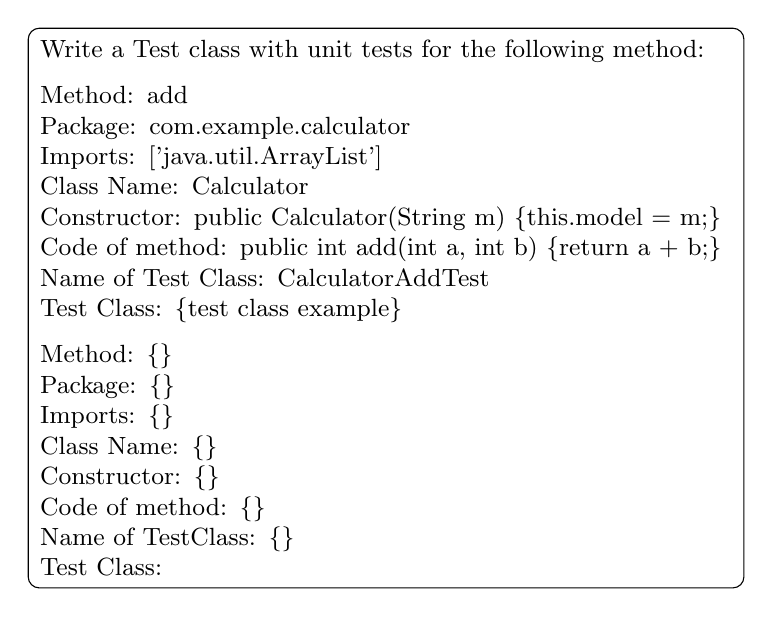
\begin{tikzpicture}
        \tikzset{node distance = 0.75cm and 1.5cm}
        % Main node with embedded tikzpicture
        \node (n1) at (0,0) [block] {
            Write a Test class with unit tests for the following method: \\[0.2cm]
            Method: add\\
            Package: com.example.calculator\\
            Imports: ['java.util.ArrayList']\\
            Class Name: Calculator\\
            Constructor: public Calculator(String m) \{this.model = m;\}\\
            Code of method: public int add(int a, int b) \{return a + b;\}\\
            Name of Test Class: CalculatorAddTest\\
            Test Class: \{test class example\}\\[0.2cm]        
            Method: \{\}\\
            Package: \{\}\\
            Imports: \{\}\\
            Class Name: \{\}\\
            Constructor: \{\}\\
            Code of method: \{\}\\
            Name of TestClass: \{\}\\
            Test Class:
};
    \end{tikzpicture}
    \caption{\textit{One-Shot} Prompt Eingabedaten (mit Zusatzkontext)}
    \label{fig:content-1}
    \vspace{-.5cm}
\end{figure}
